\section{Grundlagen der Objektorientierung}

\subsection{Elemente der objektorientierten Programmierung}
\begin{itemize}
    \item Klassen (Objekte)
    \item Vererbung
    \item Kapselung
    \item Polymorphie
\end{itemize}

\subsection{Klassen}
\begin{itemize}
    \item Klassen sind Vorlagen zur Erzeugung von Objekten.
    \item Objekte werden zur Laufzeit eines Programms erzeugt.
    \item Klassen definieren Attribute (Eigenschaften) und Methoden eines Objekts.
    \item Lokale und globale Klassen\footcite[Vgl.][S. 4]{zaidiSAPABAPObjects2019}. 
    \item Beispiel Klasse Auto
    \begin{itemize}
        \item Besitzt Attribute z. B. Farbe oder Kilometerstand
        \item Definiert Methoden wie
        \begin{itemize}
            \item Starten() - Startet den Motor
            \item TankAnzeigen() - Zeigt Füllstand des Motors
        \end{itemize}
    \end{itemize}
\end{itemize}

% Abbildung Klassendiagramm
\begin{figure}
    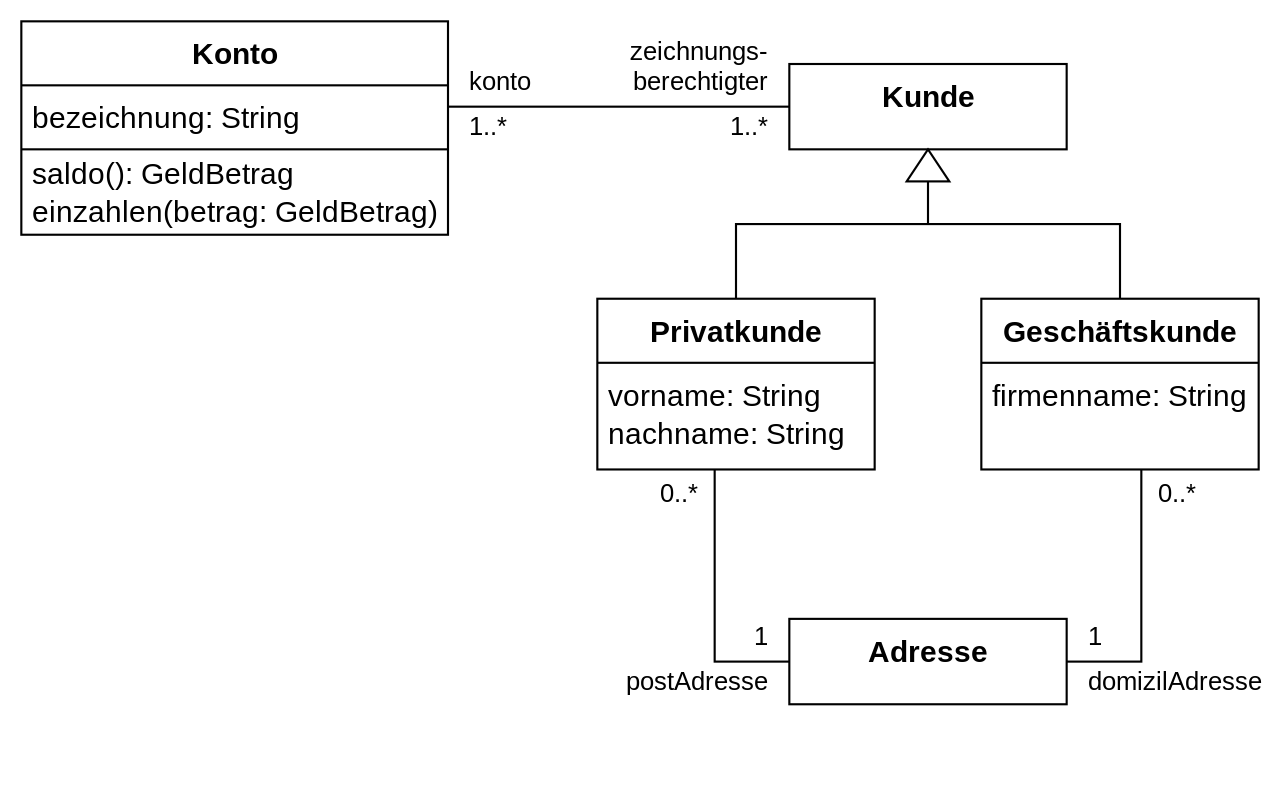
\includegraphics[width=\linewidth]{klassendiagramm}
    % Müssen wir uns nochmal anschauen, wie wir das am besten machen...
    \caption{Beispiel eines komplexeren Klassendiagramms, Quelle: \textcite{wikipediabenutzerUMLKlassendiagramm}}
    \label{fig:bsp_klassendiagramm}
\end{figure}
ABC.
\newpage